\documentclass[11pt,paper=a4,pagesize=auto,twoside,DIV=15]{scrreprt}

\usepackage[utf8]{inputenc}
\usepackage[T1]{fontenc}
\usepackage{lmodern}
\usepackage[ngerman]{babel}
\usepackage{amsmath}
\usepackage{amssymb}
\usepackage{graphicx}
\usepackage{hyperref}
\usepackage{tocloft}
\usepackage{stuff/titlepage}
\usepackage{geometry}
\usepackage{minted}
\usepackage{pgf}
\usepackage{tikz}
\usepackage{multicol}
\usepackage{multirow}
\usepackage{wrapfig}
\usepackage{todonotes}

\hypersetup{
    colorlinks=true,
    linktoc=all,
}

\recalctypearea % needed!
\newminted{python}{frame=lines,linenos,xleftmargin=5em,xrightmargin=5em}
\usetikzlibrary{arrows,automata}


\begin{document}
\begin{fullsizetitle}
\centering
\begin{minipage}{0.75\textwidth}
\vspace*{5em}
\begin{center}

\includegraphics[width=\textwidth]{images/uhh.png}\\
\vspace*{4em}
{\LARGE Universität Hamburg}\\[.25em]
{\Large Fakultät für Mathematik, Informatik und Naturwissenschaften}\\
{\Large Fachbereich Informatik}\\[3em]
{\Huge Abschlussbericht}\\[3em]

\newcommand{\HRule}{\rule{\linewidth}{0.5mm}}
\HRule\\[.4em]
{\Large%
64-189 Projekt\\%
Entwurf, Realisierung und Programmierung eines Mikrorechners\\%
Wintersemester 13/14\\%
}
\HRule\\[3em]

\begin{minipage}[t]{0.4\textwidth}
\begin{flushleft} \large
Verfasser:\\[1em]%
Marcel Hellwig\\%
Felix Ortmann\\%
David Weber\\%
Felix Wiedemann\\%
Nasif Yüksel%
\end{flushleft}
\end{minipage}
\hfill
\begin{minipage}[t]{0.4\textwidth}
\begin{flushright} \large
Betreuer:\\[1em]
Dr. Andreas Mäder\\%
Bernd Schütz%
\end{flushright}
\end{minipage} \\[12em]

{\large Vorgelegt am: \today}
\end{center}
\end{minipage}
\end{fullsizetitle}

\cleardoublepage
\tableofcontents

\cleardoublepage
\chapter{Einleitung}
% Einleitung 
Ein Computer ist keine komplizierte Maschine. Die Meisten wissen, dass er aus einem Prozessor, einem Arbeitsspeicher und einer Festplatte besteht. Der Prozessor steuert die Maschine und treibt die Datenverarbeitung voran, der Arbeitsspeicher dient als Puffer für die Aufträge und die Festplatte ist für die persistente Speicherung der Daten zuständig. Weiterhin können noch Hardwareteile wie eine Grafikkarte, ein DVD-Laufwerk oder eine Webcam verbaut sein.
Beschäftigt man sich etwas genauer mit dem Thema, wird man schnell feststellen, dass nicht all diese Komponenten zwingend notwendig sind. Dass die Webcam oder das DVD-Laufwerk nicht unbedingt zu jedem PC gehören erkennen wohl die Meisten. Dass auch die Grafikkarte und die Festplatte nicht zur Grundidee eines Computers gehören ist nicht so offensichtlich.

Der österreichisch-ungarische Mathematiker John von Neumann publizierte im Jahr 1945 eine Architektur, die die Basis moderner PCs, Laptops, Smartphones darstellt.
Die nach ihm benannte Architektur besteht aus einer Recheneinheit, der Central Processing Unit (CPU), einem Speicher für die Daten und Befehle, einer Ein- und Ausgabe-Einheit, damit der Mensch mit der Maschine interagieren kann und einem Bussystem, das die genannten Komponenten miteinander verbindet. Die CPU steuert dabei alle anderen Komponenten. Aber woher weiß die CPU, was zu tun ist? Denn der Prozessor ist auch nur ein Hardwareteil, das ohne Anweisungen nicht weiß, was zu tun ist. Eine Architektur muss die Regeln vorgeben, wie Befehle auszuführen sind. Diese Architektur bestimmt, wie schnell und effizient Befehle ausgeführt werden. Der Prozessor kann noch so modern sein, wenn die Architektur schlecht ist, wird auch der Computer keine Wunder vollbringen. Nicht umsonst verdienen Unternehmen wie Intel, AMD und neuerdings auch Qualcomm Milliarden mit dem Verkauf von Prozessoren. 
% TODO: Algorithmus -> Programm, von-Neumann vs. Harvard! 

Wie wichtig die Prozessorarchitektur ist, sieht man auch gut am Beispiel von Apple. Das Top-Smartphone von Apple läuft mit einem 1,3 GHz-Dual-Core-Prozessor. Das Top-Modell von Samsung läuft mit einem 2,5 GHz-Quad-Core-Prozessor. Dennoch laufen beide Smartphones mit einem ähnlichen Arbeitstempo und erreichen ähnliche Werte in Benchmarks. Natürlich kann man die 2 Prozessoren nicht direkt miteinander vergleichen, da es sich um andere Architekturen und Hersteller handelt. Außerdem läuft nicht das gleiche System auf beiden Geräten. Dennoch ist der Unterschied der Taktfrequenz deutlich.

Mit diesem \glqq magischen\grqq \ Algorithmus durften und mussten wir uns in dem Projekt \glqq Entwurf, Realisierung und Programmierung eines Mikrorechners\grqq \ beschäftigen. 
%TODO

\section{Das Team}
Unser Team besteht aus verschiedensten technikbegeisterten Mitgliedern. Das Softwareteam setzt sich zusammen aus Nasif Yüksel, Student der Wirtschaftsinformatik im fünften Semester.  Felix Ortmann, Student der Informatik im sechsten Semester. David Weber, Student der Wirtschaftsinformatik. Felix Wiedemann, Student der Informatik im fünften Semester. Der Hauptakteur in dem Team Hardware war Marcel Hellwig, Student der Informatik im fünften Semester.

\section{Motivation}
Zum einen waren wir einfach neugierig zu erfahren, wie die Software mit der Hardware im Detail zusammenspielt. In der Veranstaltung Rechnerstrukturen haben wir ersten Kontakt mit diesem Thema bekommen. Um unser großes Interesse weiter zu vertiefen und in die Praxis umzusetzen, hat sich dieses Projekt ideal angeboten.
Ein weiterer Grund für dieses Projekt war, dass wir unbedingt unser Projekt im Arbeitsbereich TAMS machen wollten. Denn bereits im Seminar wurden wir durch interessante Themen und einer tollen Unterstützung durch das Lehrpersonal überrascht.
Außerdem hat die Vorstellung, einen eigenen Mikrorechner zu konzipieren, jeden von uns gereizt.

\section{Material}
Um unsere Testergebnisse sichtbar zu machen, wurde ein FPGA-Prototyp, u.a. ausgestattet mit 4 LEDs, 4 Tastern, einem 800x400-Touchscreen und diversen Schnittstellen verwendet. Unser Ziel war es, die LEDs durch Drücken der Taster zum Leuchten zu bringen.
% TODO: Ziel spezifizieren

Ob das Ziel in unserem Projekt erreicht wurde, was besonders gut oder schlecht lief, was für Schwierigkeiten auftraten und welche Herausforderungen gemeistert wurden, wird auf den nächsten Seiten detailliert dargestellt. 


\chapter{Allgemein}
%general
 
\section{vorgehensweise inkl organisation}
% aufteilung in versch. gruppen
% treffen
% ticket systems, verwaltung von code, issue tracker
\section{warum python} %Ortmann
% weil myhdl (dazu kann marcel noch was sagen)
% und der rest ergab sich einfach
\section{ein wort zur lizenz} %Ortmann
% GPLv3
\section{tools}
\subsection{python}
\subsection{git}
\subsection{pycharm}
\subsection{latex}
\subsection{altera}
\subsection{hades}
\subsection{gtkwave}
\section{testen}
% unit testing





\chapter{Hardware}
\section{Modelliersprache}
Zur Beschreibung wurde, entgegen der in dem Projekt genannten Sprache, MyHDL\footnote{\url{http://myhdl.org}} genutzt. Es wurde uns von einem Kommilitonen nahe gelegt \textit{nicht} VHDL zu nutzen, da dies einen Großteil der Zeit in Anspruch nimmt die Sprache zu lernen. Diese Zeit würde später fehlen, wenn man den Mikrocontroller implementieren möchte
MyHDL ist ein Python-Modul, welches dazu genutzt wird Python als Hardwarebeschreibungssprache zu nutzen. Außerdem können damit auch Tests geschrieben werden, die zur Verifikation der Devices dient.
Ein Beispiel ist zu finden unter \autoref{HW:DFlipFop}.

\begin{figure}[h]
\small
\begin{pythoncode}
from myhdl import *
 
def dff(q, d, clk):
 
    @always(clk.posedge)
    def logic():
        q.next = d
 
    return logic
\end{pythoncode}
\caption{\label{HW:DFlipFop}D-FlipFlop}
\end{figure}

In Zeile drei werden sämtliche Ports der Komponente deklariert. Dabei werden -- im Gegensatz zu VHDL -- keine Spezifikationen wie input/output oder Bitlänge definiert. Diese werden laut Konvention nur in dem Kommentar der ``Funktion'' definiert.\\
Der Dekorator\footnote{\url{https://wiki.python.org/moin/PythonDecorators}} in Zeile 5 wird benutzt um zu spezifizieren, wann die dekorierte Funktion ausgeführt werden soll. In diesem Falle wird gesagt, dass bei einer steigenden Flanke des clk-Ports die Funktion ausgeführt werden soll.\\
Die eigentliche Logik der Komponente befindet sich in Zeile 7. Hier wird gesagt, dass im nächsten Augenblick der Wert von \textit{q d} sein soll.
In Zeile 9 wird die dekorierte Funktion zurückgegeben, d.h. sie wird in der Simulation und Transformation berücksichtigt.\\
Gut zu sehen sind an diesem Beispiel die Vor- und Nachteile von Python als Hardwarebeschreibungssprache. Ein Nachteil ist, dass man die genaue Spezifikation eines Ports nicht direkt angeben kann, z.B. deren Bitweite oder Typ. Dies kann zu Fehlern führen und zu viel Frust. MyHDL entscheidet die Eigenschaften durch statische Analyse des Quellcodes.\\
Vorteile hingegen sind der große Umfang der Python-Bibliotheken, die man sehr gut zum Testen der Komponenten nutzen kann, z.B. reguläre Ausdrücke, Listen oder Hashmap, sowie die einfache Erlernbarkeit und viele Syntaktische Feinheiten.\\

\section{Design}
\begin{figure}
\vspace{-4em}
\centering
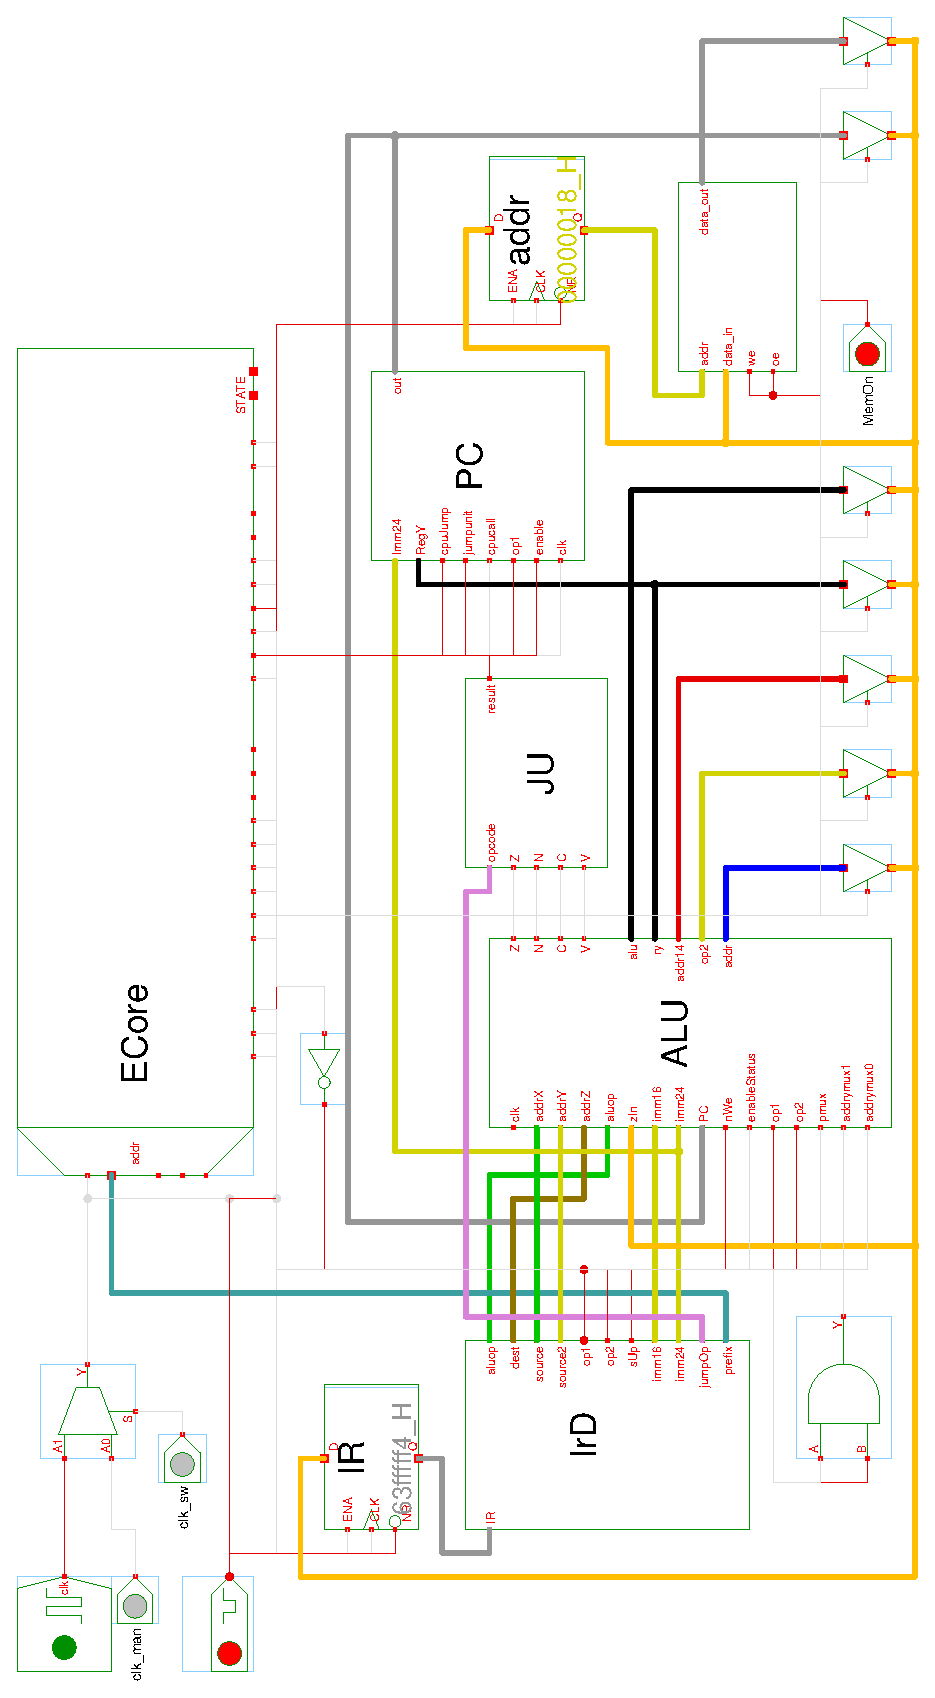
\includegraphics[width=.8\textwidth]{images/overview.eps}
\caption{\label{HW:Overview}Übersicht des MK}
\end{figure}
Das Design der Mikrocontrollers ist sehr stark am D-Core\footnote{\url{http://tams-www.informatik.uni-hamburg.de/applets/hades/webdemos/60-dcore/t3/processor.html}} orientiert, mit einem zentralen Bus, einem Steuerwerk, einer Abstraktion für den Speicher, sowie Elementen, die mit Hilfe des Busses miteinander kommunizieren. Wie man in der \autoref{HW:Overview} sehr gut sehen kann ist die Verbindung zwischen den einzelnen Komponenten auf ein Minimum gehalten. Einzige Ausnahme bildet hierbei der Instruction-Decoder. Auf die einzelnen Komponenten wird in den Folgenden Abschnitten noch genauer eingegangen.\\
Die Entscheidung zu dieser Anordnung kam aus der Überlegung heraus, dass wir uns an etwas bestehendem orientieren wollten. Deswegen ist verfügt er über einen Bus und verschiedene TriState-Dioden, die von einer Zentralen Einheit angesteuert werden, in unserem Fall das Steuerwerk oder CPU genannt. Doch genau hier liegt auch das Problem, denn die CPU ist nicht in der Lage aktiv werte an Komponenten zu senden, sondern schaltet nur Leitungen an oder aus. Auf dieses Problem wird später in der ALU auch noch genauer eingegangen. So gibt es an einigen Stellen für bestimmte Probleme maßgeschneiderte Lösungen.\\
Ein dennoch großer Vorteil eines gemeinsamen Busses ist die einfache Erweiterbarkeit des Systems. So hatten wir am Anfang gar nicht mit einer RS232-Schnittstelle gerechnet, konnte diese später jedoch Problemlos einfügen, indem sie am Bus lauscht/schreibt und von der CPU geschaltet wird.\\
Die eigentliche Beschreibung des Mikrocontrollers erfolgt letztendlich in Python und kann im Beigelegten Projektordner eingesehen werden.

\subsection{Steuerwerk}
Unser Steuerwerk (CPU) ist eine State-Maschine (\ref{HW:CPU-State}), die anhand eines Präfix in den nächsten Status gelangt. In einem Status ist genau festgehalten zu welchem Zeitpunkt welche Steuerleitung (de-)aktiviert wird. Hier ist es möglich Substates zu haben (realsiert mit Hilfe eines hochlaufen Counters), falls dieser Befehl mehr als einen Takt benötigt um z.B. auf die Antwort der MMU zu warten. Das Bereit sein wird asynchron gemeldet, das heißt über eine eingehen Steuerleitung. 

\begin{figure}[h]
TODO: state chart machen
\begin{tikzpicture}[semithick]
    \tikzstyle{every state}=[fill=white,draw=none,text=black]
    \node[initial,state]    (F)                        {$Fetch$};
    \node[state]            (D)    [below of=F]        {$Decode$};
    
    \path[->] (F)     edge    node {}    (D);
\end{tikzpicture}
\caption{\label{HW:CPU-State}Cpu}
\end{figure}

\subsection{Instruction Decoder}
Der Instruction Decoder (IrD) ist zuständig dafür, einen 32Bit langen Wert in seine Einzelteile zu zerlegen und den einzelnen Komponenten zur Verfügung zu stellen. Dies soll ohne Takt geschehen, sondern sofort. Eine Entsprechende Abbildung ist unter \autoref{HW:IRD} zu sehen.\\
\begin{figure}[h]
\centering
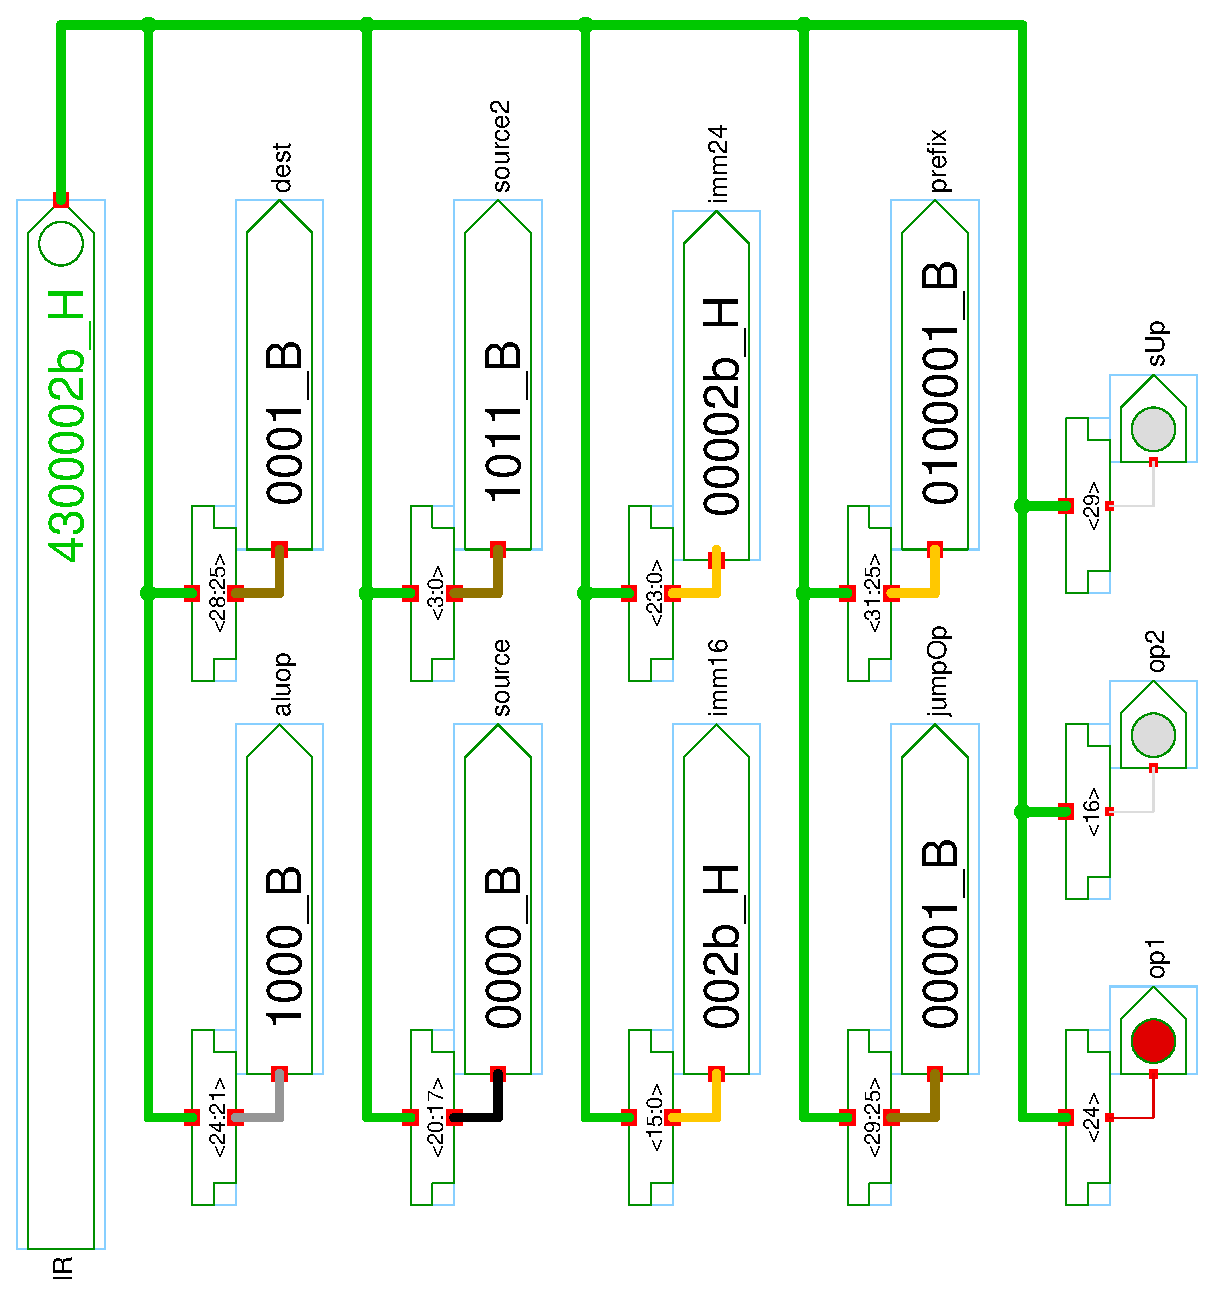
\includegraphics[width=.8\textwidth,angle=270]{images/ir.eps}
\caption{\label{HW:IRD}Instruction Decoder}
\end{figure}
Der IrD stellt 8 Werte bereit und 3 Flags. Die Einzelnen Werte stehen für:

\begin{itemize}
  \item aluop -- Der Op-code für die ALU
  \item dest --  Die Zieladresse für die Registerbank (Z)
  \item source -- Die Quelladresse für die Registerbank (X)
  \item source2 -- Die zweite Quelladresse für die Registerbank (Y)
  \item imm16 -- Ein 16Bit breiter Immediate Wert für Berechnungen
  \item imm24 -- Ein 24Bit breiter Immediate Wert für Berechnungen
  \item jumpop -- Der Op-code für die Sprungeinheit.
  \item prefix -- Das Instruktionsprefix für die CPU
\end{itemize}
Mit Hilfe der einzelnen Werte und Flags ist es nun möglich einen Befehl gemäß unserer Befehlsstruktur auszuführen. Da Werte nicht immer sinnig sein müssen, z.B. bei einem Sprungbefehl kann ein unsinniger Aluop entstehen, ist für die Hardware nicht weiter schlimm. Denn die berechnet einfach, wird ihr Ergebnis aber nie auf den Bus schreiben, denn die CPU unterbindet dies.
\subsection{ALU}
\begin{figure}[h]
\centering
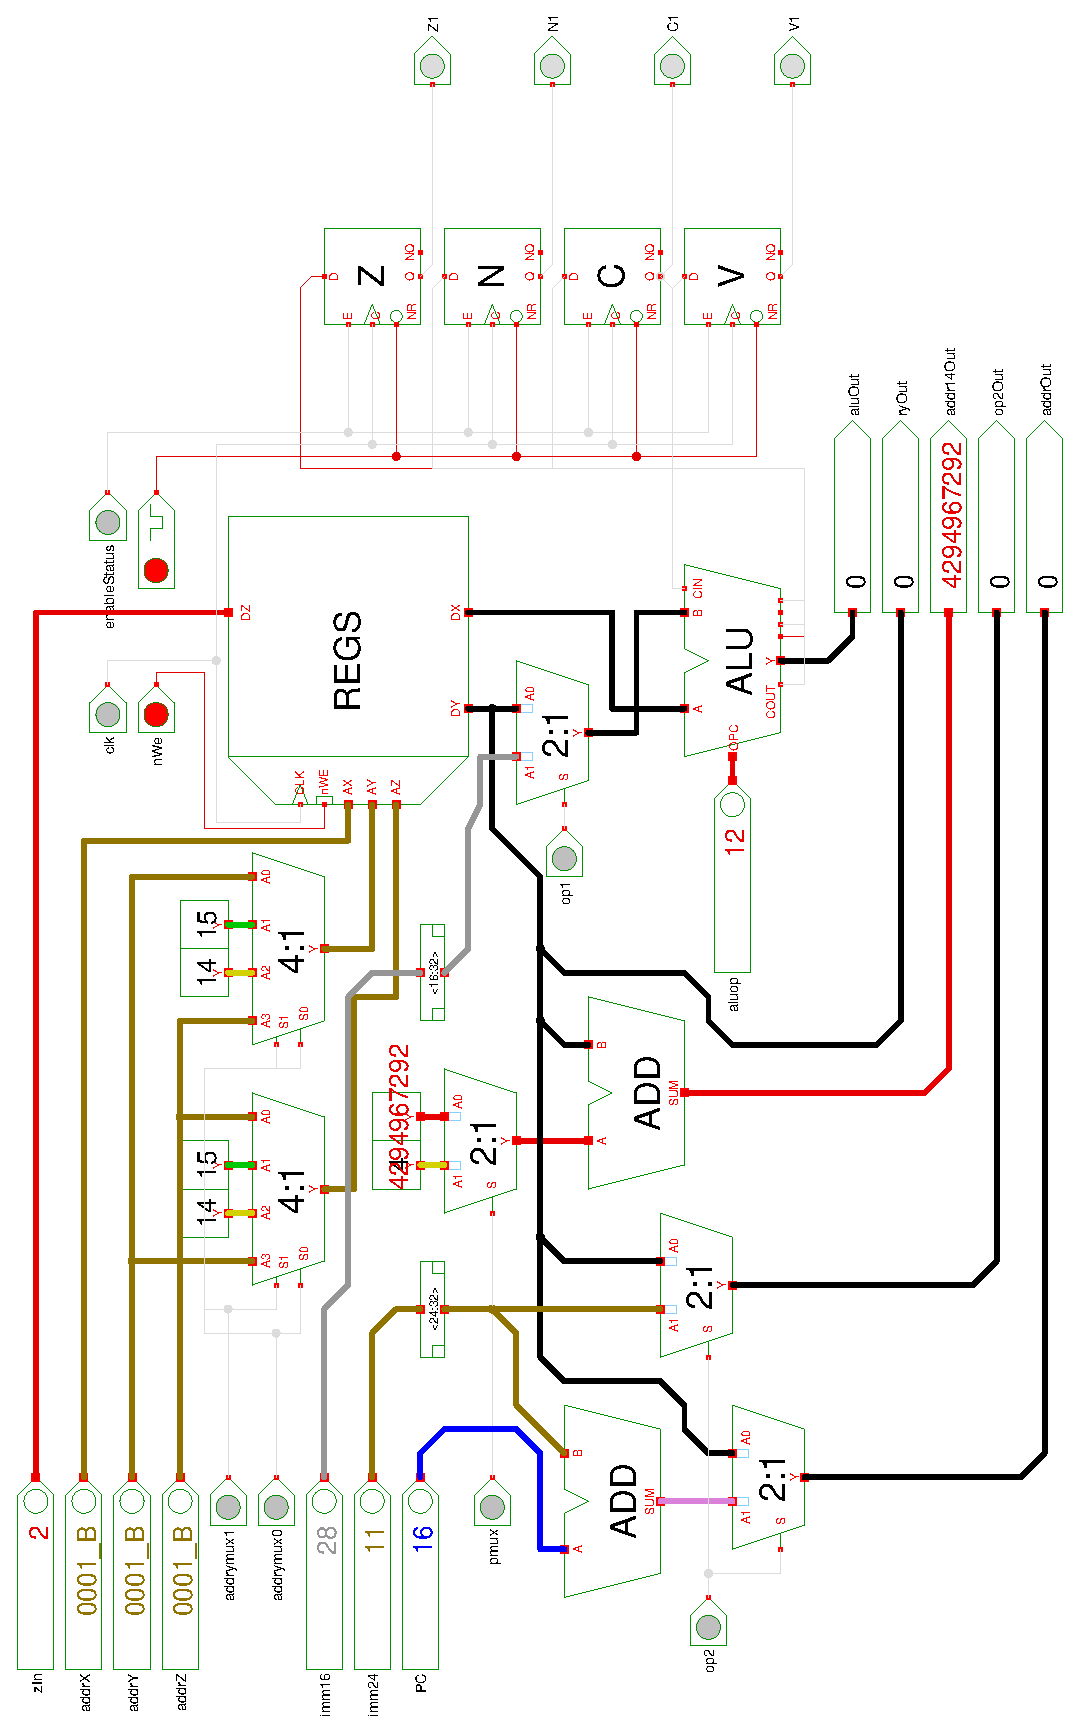
\includegraphics[width=.8\textwidth]{images/alu.eps}
\caption{\label{HW:ALU}Address, Arithmetisch und Logische Einheit}
\end{figure}
\subsection{Jumpunit}
\begin{figure}[h]
\centering
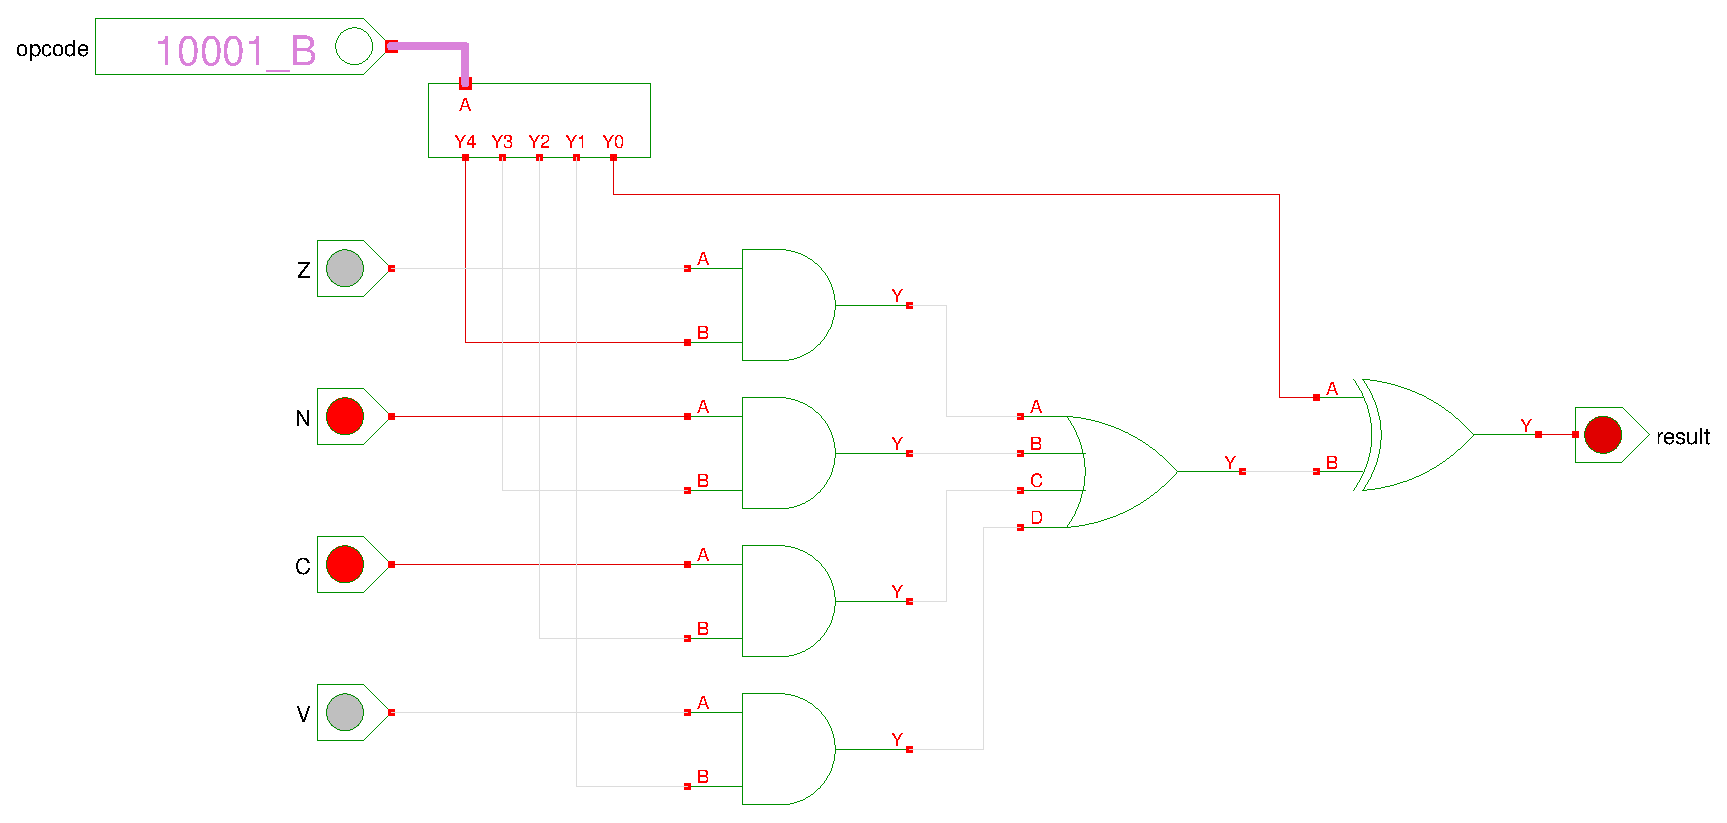
\includegraphics[width=1\textwidth]{images/ju.eps}
\caption{\label{HW:JU}Sprung-Einheit}
\end{figure}
\subsection{Programmcounter}
\begin{figure}[h]
\centering
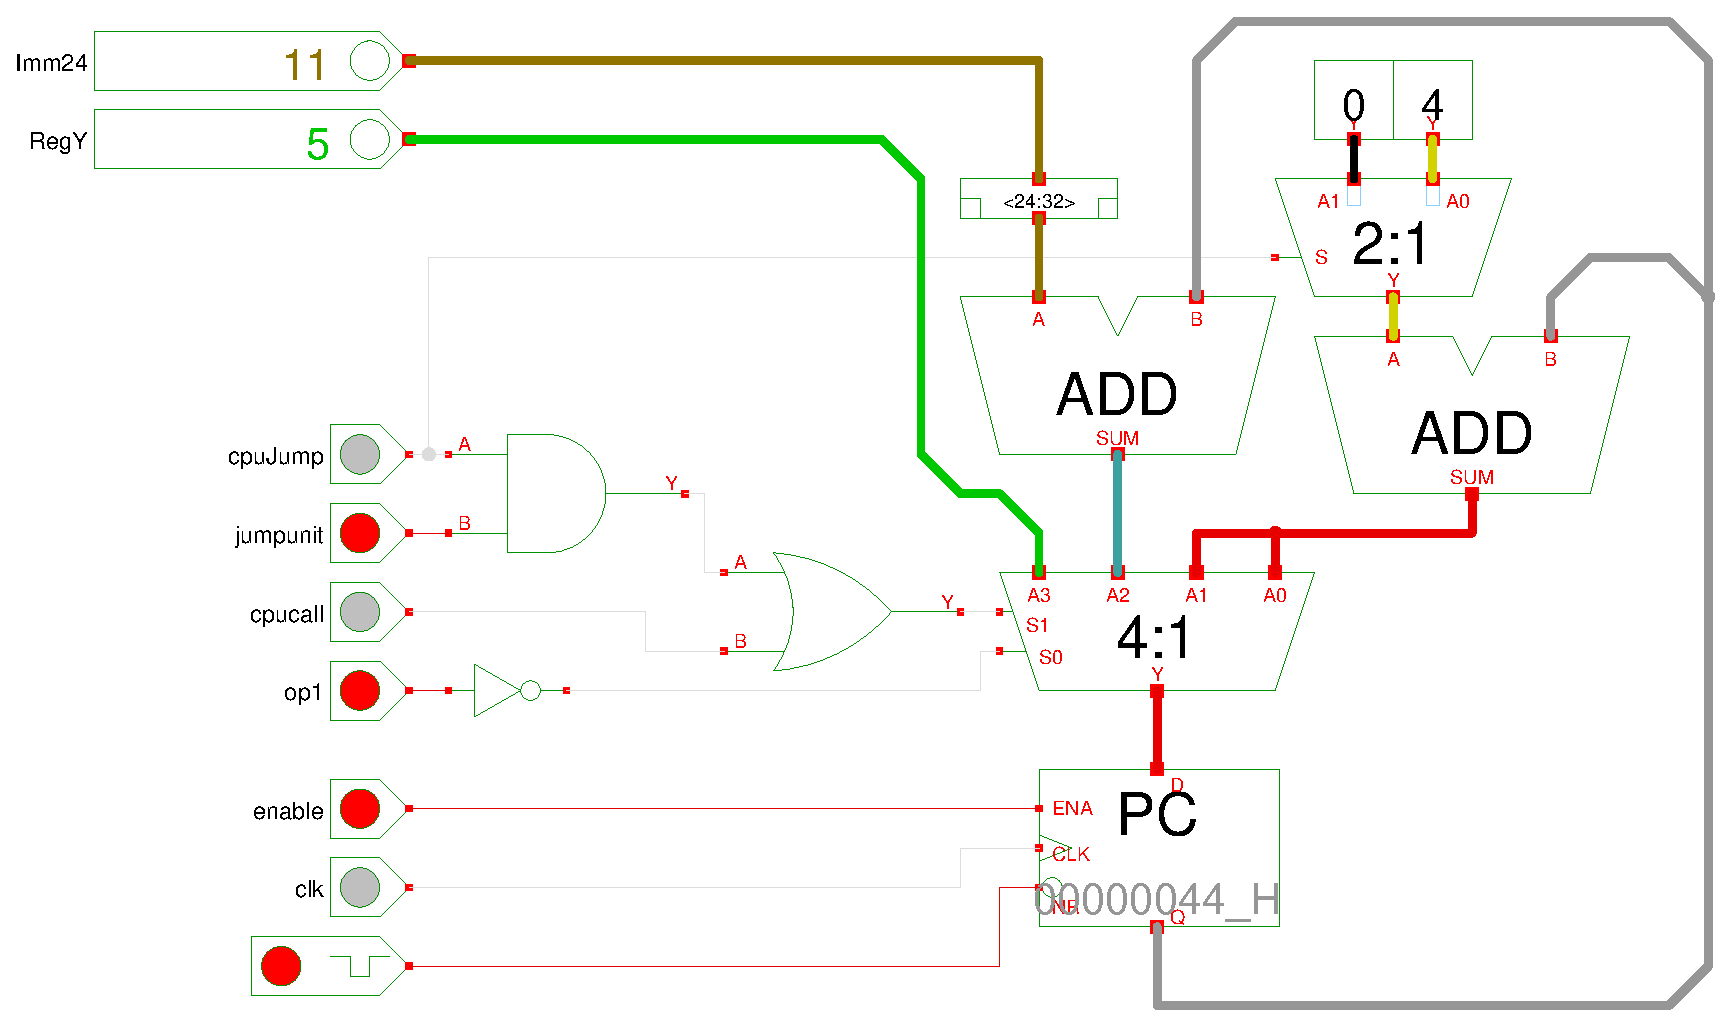
\includegraphics[width=1\textwidth]{images/pc.eps}
\caption{\label{HW:PC}Programmcounter}
\end{figure}
\subsection{Memory}


\chapter{Software}

\section{ISA} % Felix ?., Marcel
% TODO: RISC, Wortbreite, Registeranzahl, GP-Regs, SP und PC als GP ausgelegt, …
Den Aufbau unserer Instrution Set Architecture haben wir bereits beim ersten Gruppentreffen begonnen und stark umstritten. Im Verlauf des Projekts hat sich viel geändert, zum Teil motiviert durch Wünsche und Verbessungsideen unserer Mitglieder, zum Teil begründet in Fehlern oder Problemen mit den Befehlsworten oder deren Bitcode-Layout.
In der \autoref{AP:ISA} ist unsere endgültige Instruction Set Architecture zu sehen. Wir haben von Beginn an den Fokus auf eine überschaubare Komplexität gelegt. Unsere arithmetischen Operationen zum Beispiel enthalten nur Befehle für Addition, Subtraktion und Multiplikation. Division haben wir nicht behandelt, da das ein tiefergehendes Auseinandersetzen mit Gleitkommazahlen nach sich gezogen hätte. \todo{Das ist Quark, +1} Gleitkomma-Arithmetik haben wir von Beginn an als schwieriges, nicht notwendiges Feature eingestuft. \todo{Spezialitäten von ARM und MIPS abgekupfert: \$0, Statusflag}

Für die Speicherzugriffsbefehle nutzen wir lediglich kustomisierte Varianten von load und store. Bemerkenswert ist jedoch unser breites Angebot an Sprungbefehlen. Diese haben wir so definiert, dass sie auf Labels referenzieren können. \todo{Ungenau, sind 'nur' pc-relative Sprünge; nothing special here} Labels sind in unserem Assembler Punkte im Code, die einen funktional zusammengehörigen Block markieren. Dies war am Anfang des Semesters noch völlig offen und hat sich erst mit der Zeit ergeben. Die Verwendung von Labels hatten wir zunächst, ähnlich wie die Gleitkomma-Arithmetik, als nicht so wichtig eingestuft. Für viele Programmabläufe sind Sprünge jedoch unabdingbar und daher umso dringender als Kommando im Assembler benötigt. Das endgültige Design der Springbefehle ist derart gestaltet, dass sie konditionierbar sind; die bekannte Befehle, die bei einer Vergleichsoperation ausgelöst werden können, etwa jump-less-or-equal, haben wir um Befehle erweitert, die auf jedem Statusflag-Status unserer ALU aufsetzen. So gibt es beispielsweise einen Jump-Befehl für den Overflow Fall, der aus Rahmen eines herkömmlichen Minimalassemblers herausfällt.
Schlussendlich haben sich in unserer ISA auch noch Befehle als nützlich erwiesen, die eine spezielle Funktion direkt an der Hardware abstrahieren. Die ISA bietet uns die Möglichkeit direkt auf Buttons und LEDs auf dem FPGA zuzugreifen und diese Hardwarelemente in logisch unären Operationen anzusprechen. Dies ist sehr praktisch, denn eine Abfrage der Buttonelemente für jedes Programm als Sprachkonstrukt in herkömmlichem Assembler implementieren zu müssen, erschien uns sehr umständlich.

All diese Feinheiten der ISA haben sich mit der Zeit entwickelt. Beginnend bei unserem Primärziel, ein FPGA zu einem kleinen Taschenrechner werden lassen, hatten wir eine entsprechend kleine ISA. Sie umfasste lediglich den Befehlsatz für arithmetische Operationen, der fast genau so bis zur endgültigen ISA geblieben ist, Kontrollfluss regulierende Befehle wie call und jump, die wir zu diesem Zeitpunkt noch nicht weiter durchdacht hatten, sowie einen load und store Befehl. Wie \autoref{AP:ISA} zeigt, hat sich die ISA im Vergleich zu \autoref{gen:Idee} stark erweitert. \todo{calculator.s in Anhang und referenzieren}

% TODO: entwicklung zur final isa
% probleme am anfang
% probleme zwischendurch
% geil am ende

\section{ABI}
% TODO

\section{Assembler} % Felix W.
% TODO: do your shit
% inkl. programmbeispiele
% faculty.s mit Kommentaren

\section{Emulator} % Felix W.
% TODO: do your shit

\section{GUI/Debugger(Marcel)}
% TODO: do your shit

% TODO: calculator.s mit Kommentaren im Anhang


\chapter{Fazit}
%fazit

\section{Ergebnisse}
% voll funktionsfähiger prototyp
% sogar mit fpga ding
% 'über das ziel hinausgeschossen'

\section{Probleme} %0ortmann

\subsection{Gruppe \todo{hier evtl nicht gliedern}}
Zu Beginn unseres Projektes bestand die Gruppe aus 7 Mitgliedern, die sich nach recht kurzer Zeit um zwei reduziert hat. Schade war, dass die Mitglieder nicht einfach ausgetreten sind, sondern bis zum Ende trotz wiederholten Anfragen einfach nichts getan haben. Im Folgenden ist mit \textit{unserer Gruppe} also das reduzierte Team von 5 Leuten gemeint.
Im Verlauf underes Projektes haben sich über die Zeit einige Probleme ergeben. Dies war meist begründet durch kurzfristig nötige Programmänderungen, die dann zu größeren Diskussionen führten. Im Allgemenein hat unsere Gruppe dazu geneigt, Einzelheiten sehr fein auszudiskutieren. Auch bei der vielfältigen Änderung unserer ISA, siehe auch das zugehörige Kapitel, hat sich einiges an Streitigkeiten ergeben. Besonders anzumerken ist jedoch, dass alle Streitigkeiten in unserer Gruppe stets fachlich begründet waren. Unsere Mitglieder haben sich nicht etwa aus persönlichen Gründen nicht verstanden, sondern hatten vielmehr alle immer konstruktiv etwas zu den Fragestellungen beizutragen und daraus ergaben sich dann größere Diskussionen.

\subsection{Fachliche Probleme}
Wie auch schon im Kapitel ISA kurz angerissen wurde, ergaben sich vielfältige Änderungen an der Befehlsstruktur. Zunächst hatten wir nur ein sehr begrenztes Befehlset, am Ende auch Befehle zum direkten Ansteuren von Hardwareelementen. Die Problematik dahinter lag in der Hardware des FPGA begründet. 
Ein bis jetzt bestehendes Problem unserer Architektur ist, dass unser Microcontroller kein byteweises Laden und Speichern unterstüztz. Auch Kommunikationsmanagement bzw. Nachrichtenaustauschürotokolle unterstrützt der Controller nicht und dementsprechend kennt er auch keine Interrupts.


% isa musste mehrfach angepasst werden
% |- weil moppelkotze
% |- weil hardware dumm
% bestehende probleme
% |- kein byteweises laden/speichern
% intergruppendynamikkommunikationsaustauschverhalten
% sven und alisa sind rausgeflogen

\section{Erkenntnisse}
% TODO: hardware designen ist nicht schwer
% man muss sich nur gedanken machen
% verständniss für hardware wurde verbessert
% verständniss für software wurde verbessert
% gruppenarbeit ist wichtig und toll
% issue tracker nutzen um übersicht zu behalten
% git ist toll

\section{Ausblick} %1hellwig
% was könnten wir noch machen
% |- video
% |- audio
% |- pipeline
% |- cache
% |- interrupts
% |- multi threading ...
% assembler (siehe github)

\section{Fazit}
% TODO: war super
% machen wir gern noch mal
% wir sehen uns im master


\chapter{Appendix}
\section{Ideensammlung}
\centering
\vspace*{-12em}
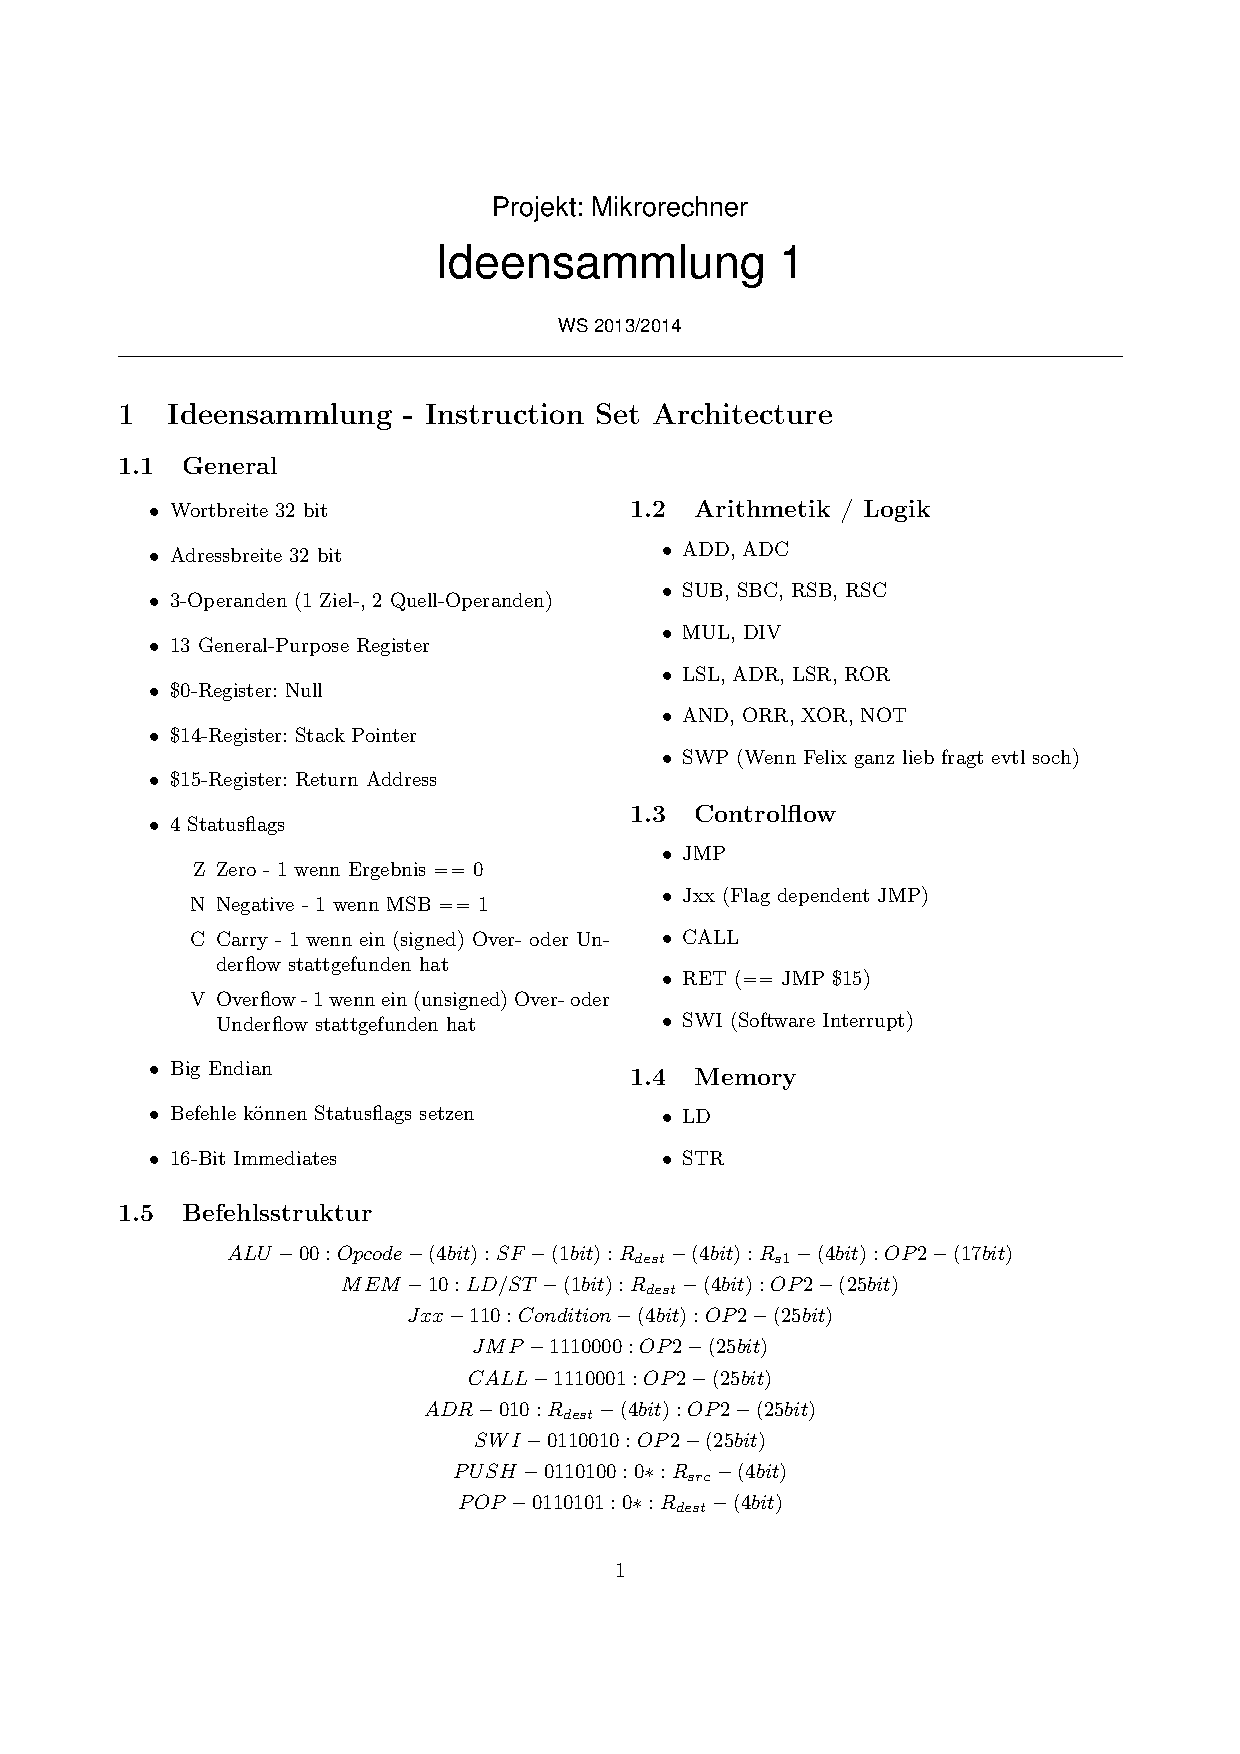
\includegraphics[width=\textwidth]{images/Ideensammlung.pdf}
\vspace*{-7em}
\captionof{figure}{\label{gen:Idee} Ideensammlung}
%TODO: FIXME: Abbildungsbeschreibung landet auf der nächsten Seite
\section{ISA}
\begin{table}[H]
\label{isatable}
\hspace{1em}
\texttt{
\begin{tabular}{|p{2cm}|l|l|l|}
\hline
\multirow{7}{*}{\textbf{Arithmetic}} & Add & add \$d, \$s, \$t & 00 S dddd 0000 ssss op3 \\ \cline{ 2- 4}
 & Addc & adc \$d, \$s, \$t & 00 S dddd 0001 ssss op3 \\ \cline{ 2- 4}
 & Sub & sub \$d, \$s, \$t & 00 S dddd 0100 ssss op3 \\ \cline{ 2- 4}
 & Subc & sbc \$d, \$s, \$t & 00 S dddd 0101 ssss op3 \\ \cline{ 2- 4}
 & Revsub & rsb \$d, \$s, \$t & 00 S dddd 0110 ssss op3 \\ \cline{ 2- 4}
 & Revsubc & rsc \$d, \$s, \$t & 00 S dddd 0111 ssss op3 \\ \cline{ 2- 4}
 & Mul & mul \$d, \$s, \$t & 00 S dddd 0010 ssss op3 \\ \hline
\multirow{5}{*}{\textbf{Logical}} & And & and \$d, \$s, \$t & 00 S dddd 1000 ssss op3 \\ \cline{ 2- 4}
 & Andn & adn \$d, \$s, \$t & 00 S dddd 0011 ssss op3 \\ \cline{ 2- 4}
 & Or & orr \$d, \$s, \$t & 00 S dddd 1001 ssss op3 \\ \cline{ 2- 4}
 & Xor & xor \$d, \$s, \$t & 00 S dddd 1010 ssss op3 \\ \cline{ 2- 4}
 & Orn & orn \$d, \$s, \$t & 00 S dddd 1011 ssss op3 \\ \hline
\multirow{4}{*}{\parbox{2cm}{\textbf{Shift / Rotate}}} & lsl & lsl \$d, \$s, \$t & 00 S dddd 1100 ssss op3 \\ \cline{ 2- 4}
 & asr & asr \$d, \$s, \$t & 00 S dddd 1101 ssss op3 \\ \cline{ 2- 4}
 & lsr & lsr \$d, \$s, \$t & 00 S dddd 1110 ssss op3 \\ \cline{ 2- 4}
 & ror & ror \$d, \$s, \$t & 00 S dddd 1111 ssss op3 \\ \hline
%
\multirow{12}{*}{\textbf{Jump}} & Jump & jmp .label & 01 00001 op2 \\ \cline{ 2- 4}
 & Jump & jmp op2 & 01 00001 op2 \\ \cline{ 2- 4}
 & Jump Equal & jeq .label & 01 10000 op2 \\ \cline{ 2- 4}
 & Jump Not Equal & jne .label & 01 10001 op2 \\ \cline{ 2- 4}
 & Jump Less Than & jlt .label & 01 01000 op2 \\ \cline{ 2- 4}
 & Jump Less Equal & jle .label & 01 11000 op2 \\ \cline{ 2- 4}
 & Jump Greater Than & jgt .label & 01 11001 op2 \\ \cline{ 2- 4}
 & Jump Greater Equal & jge .label & 01 01001 op2 \\ \cline{ 2- 4}
 & Jump Overflow & jo \ .label & 01 00010 op2 \\ \cline{ 2- 4}
 & Jump Not Overflow & jno .label & 01 00011 op2 \\ \cline{ 2- 4}
 & Jump Carry & jc \ .label & 01 00100 op2 \\ \cline{ 2- 4}
 & Jump Not Carry & jnc .label & 01 00101 op2 \\ \hline
\multirow{3}{*}{\textbf{Memory}} & Load & ld \$d, \$s & 100 dddd op2 \\ \cline{ 2- 4}
 & Store & st \$d, \$s & 101 dddd op2 \\ \cline{ 2- 4}
 & adr & adr \$d, \#imm & 110 dddd * imm24 \\ \hline
\multirow{2}{*}{\parbox{2cm}{\textbf{Push / Pop}}} & Push & push \$s & 11100 \ \ \ * op2 \\ \cline{ 2- 4}
 & Pop & pop \$d & 11101 \ \ \ * op2 \\ \hline
\multirow{6}{*}{\textbf{Special}} & Call & call .label & 111100 \ \ * op2 \\ \cline{ 2- 4}
 & Clock & clk \$d & 111101 \ \ * dddd \\ \cline{ 2- 4}
 & Get Button & but \$d & 1111100 \ * dddd \\ \cline{ 2- 4}
 & Set Led & led \$l & 1111101 \ \ \ op2 \\ \cline{ 2- 4}
 & Rs232 read & rsr \$d & 1111110 \ * dddd \\ \cline{ 2- 4}
 & Rs232 transmit & rst \$d & 1111111 \ \ \ op2 \\ \hline
\end{tabular}
}
\caption{ISA}
\label{AP:ISA}
\end{table}

\section{Abbildungsverzeichnis}
\listoffigures 

\section{Tabellenverzeichnis}
\listoftables

\end{document}
